\documentclass[conference]{IEEEtran}
\IEEEoverridecommandlockouts
% The preceding line is only needed to identify funding in the first footnote. If that is unneeded, please comment it out.
\usepackage{cite}
\usepackage{amsmath,amssymb,amsfonts}
\usepackage{algorithmic}
\usepackage{graphicx}
\usepackage{textcomp}
\usepackage{xcolor}
\usepackage{url}
\usepackage{multicol}
\usepackage{array}
\usepackage{float} % Add the float package for H specifier
\def\BibTeX{{\rm B\kern-.05em{\sc i\kern-.025em b}\kern-.08em
    T\kern-.1667em\lower.7ex\hbox{E}\kern-.125emX}}
\usepackage{listings}
\lstset{
basicstyle=\small\ttfamily,
columns=flexible,
breaklines=true
}
\begin{document}
\onecolumn
\title{CSC 693 - HW 2 - Word2Vec Neural Network}
\author{Sahil Dhawan}
\maketitle
\section{Word Embedding}
\noindent Word embeddings are a form of word representation that bridges the human understanding of language to that of a machine using vectors. Use \textbf{all the 2,000 comments} as the corpus, and choose Gensim, GloVe or other related python libraries to finish the following tasks.
\begin{enumerate}
\item Train word embeddings vectors using word2vec method with CBOW style (vector\textunderscore size=100, window=5, min\textunderscore count=1). Report your computer’s parameters (or Google Colab) and the time used for training.\\
Computer Parameters:
\begin{itemize}
\item Lenovo Yoga 920-13IKB
\item Processor Intel Core i5-8250U @ 1.6GHz $\times$ 8
\item Ubuntu 22.04.4 LTS
\item 64-bit
\end{itemize}
After being loaded into separate lists, the positive and negative comment data was combined into one list, \verb"all_data", by appending the negative data after the positive data. \verb"all_data" was preprocessed by tokenizing each comment into words and excluding stop words and punctuation. Using \verb"all_data" and word2vec with CBOW, the time to train 2,000 comments was 5.888 seconds.\\
\begin{center}
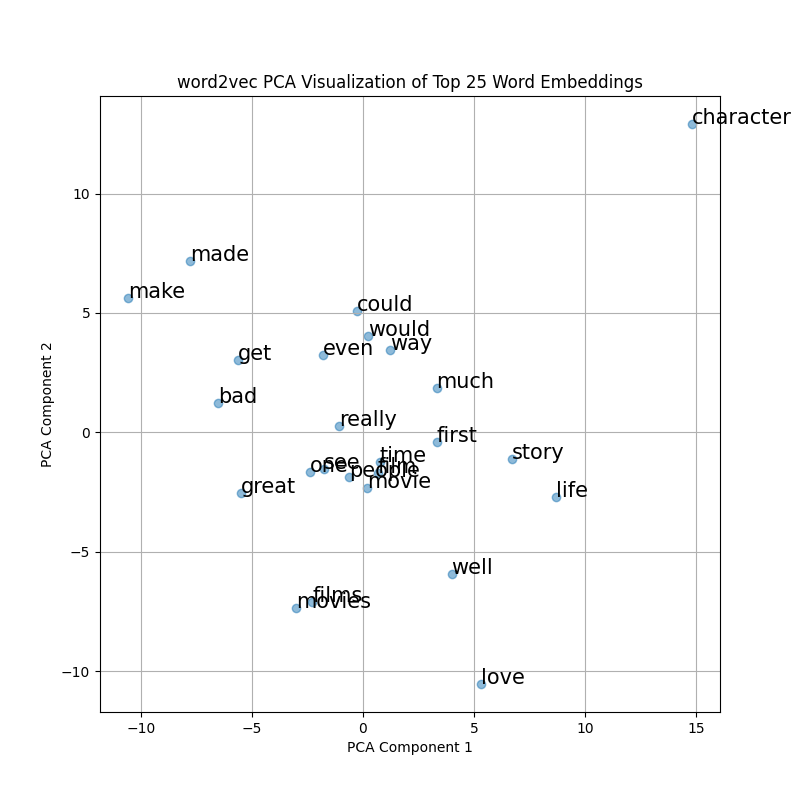
\includegraphics[scale=0.35]{word2vec Top 25 Vectors.png}
\end{center}
\newpage
\item Train word embeddings vectors using GloVe method. (vector\textunderscore  size=100, window\textunderscore size=5, vocab\textunderscore min\textunderscore count=1)\\
With the same preprocessing as 1), the time to train was 30.933 seconds.\\
\begin{center}
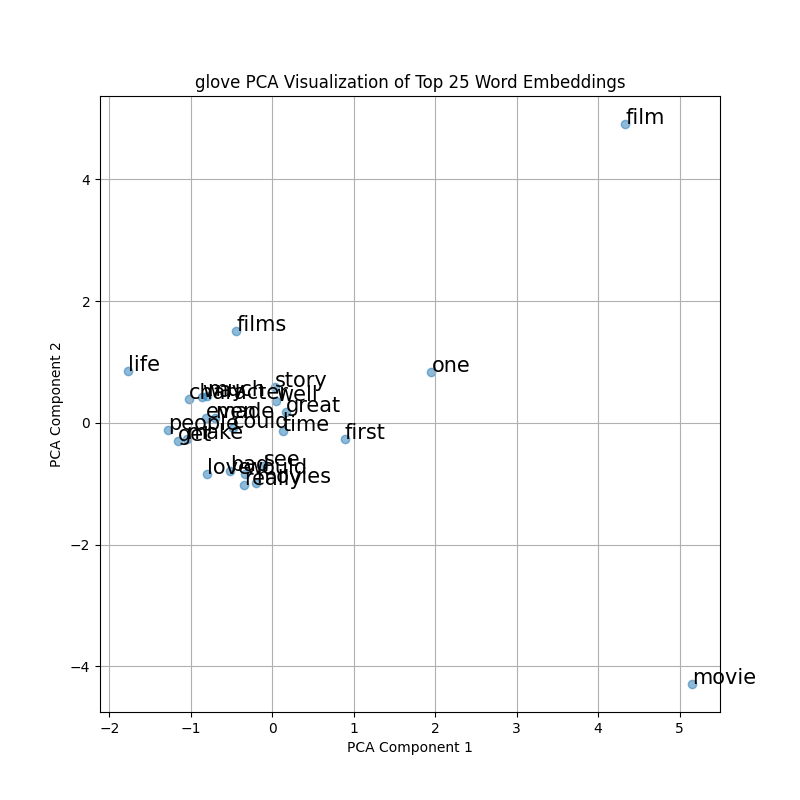
\includegraphics[scale=0.35]{glove Top 25 Vectors.png}
\end{center}
\item Evaluate the model trained in 1) and 2) by analyzing the 10 most similar words to each of the following word: “movie”, “music”, “woman”, “Christmas”. Which model’s output looks more meaningful?
\begin{table}[H]
\centering
\begin{tabular}{|llllllll|}
\hline
\multicolumn{8}{|c|}{Most Similar Words with word2vec with CBOW (vector\textunderscore size=100, window=5, min\textunderscore count=1)}                                                                                                                                                   \\ \hline
\multicolumn{2}{|c|}{movie}                               & \multicolumn{2}{c|}{music}                    & \multicolumn{2}{c|}{woman}                    & \multicolumn{2}{c|}{christmas} \\ \hline
\multicolumn{1}{|l|}{film} & \multicolumn{1}{l|}{62.00\%} & \multicolumn{1}{l|}{soundtrack} & \multicolumn{1}{l|}{72.29\%} & \multicolumn{1}{l|}{maiden} & \multicolumn{1}{l|}{72.19\%} & \multicolumn{1}{l|}{carol} & \multicolumn{1}{l|}{75.09\%} \\
\multicolumn{1}{|l|}{movies} & \multicolumn{1}{l|}{58.16\%} & \multicolumn{1}{l|}{dancing} & \multicolumn{1}{l|}{70.96\%} & \multicolumn{1}{l|}{organs} & \multicolumn{1}{l|}{67.64\%} & \multicolumn{1}{l|}{ghost} & \multicolumn{1}{l|}{73.29\%} \\
\multicolumn{1}{|l|}{stardust} & \multicolumn{1}{l|}{55.11\%} & \multicolumn{1}{l|}{songs} & \multicolumn{1}{l|}{68.52\%} & \multicolumn{1}{l|}{naive} & \multicolumn{1}{l|}{67.53\%} & \multicolumn{1}{l|}{holiday} & \multicolumn{1}{l|}{71.25\%} \\
\multicolumn{1}{|l|}{it} & \multicolumn{1}{l|}{54.98\%} & \multicolumn{1}{l|}{singing} & \multicolumn{1}{l|}{68.24\%} & \multicolumn{1}{l|}{aged} & \multicolumn{1}{l|}{66.78\%} & \multicolumn{1}{l|}{croc} & \multicolumn{1}{l|}{65.85\%} \\
\multicolumn{1}{|l|}{valentine} & \multicolumn{1}{l|}{54.55\%} & \multicolumn{1}{l|}{costumes} & \multicolumn{1}{l|}{66.43\%} & \multicolumn{1}{l|}{girl} & \multicolumn{1}{l|}{66.53\%} & \multicolumn{1}{l|}{crypt} & \multicolumn{1}{l|}{65.61\%} \\
\multicolumn{1}{|l|}{lyrics} & \multicolumn{1}{l|}{54.53\%} & \multicolumn{1}{l|}{editing} & \multicolumn{1}{l|}{66.07\%} & \multicolumn{1}{l|}{widow} & \multicolumn{1}{l|}{66.37\%} & \multicolumn{1}{l|}{festivities} & \multicolumn{1}{l|}{61.17\%} \\
\multicolumn{1}{|l|}{slur} & \multicolumn{1}{l|}{54.29\%} & \multicolumn{1}{l|}{dance} & \multicolumn{1}{l|}{65.81\%} & \multicolumn{1}{l|}{warthog} & \multicolumn{1}{l|}{65.61\%} & \multicolumn{1}{l|}{woodward} & \multicolumn{1}{l|}{61.09\%} \\
\multicolumn{1}{|l|}{thats} & \multicolumn{1}{l|}{54.23\%} & \multicolumn{1}{l|}{noises} & \multicolumn{1}{l|}{65.30\%} & \multicolumn{1}{l|}{gigi} & \multicolumn{1}{l|}{65.18\%} & \multicolumn{1}{l|}{glib} & \multicolumn{1}{l|}{59.32\%} \\
\multicolumn{1}{|l|}{tensed} & \multicolumn{1}{l|}{54.08\%} & \multicolumn{1}{l|}{photography} & \multicolumn{1}{l|}{64.87\%} & \multicolumn{1}{l|}{herding} & \multicolumn{1}{l|}{65.11\%} & \multicolumn{1}{l|}{1984} & \multicolumn{1}{l|}{58.94\%} \\
\multicolumn{1}{|l|}{swede} & \multicolumn{1}{l|}{53.64\%} & \multicolumn{1}{l|}{rap} & \multicolumn{1}{l|}{64.16\%} & \multicolumn{1}{l|}{daughter} & \multicolumn{1}{l|}{64.39\%} & \multicolumn{1}{l|}{version} & \multicolumn{1}{l|}{57.72\%} \\ \hline
\end{tabular}
\end{table}
\begin{table}[H]
\centering
\begin{tabular}{|llllllll|}
\hline
\multicolumn{8}{|c|}{Most Similar Words with GloVe (vector\textunderscore  size=100, window\textunderscore size=5, vocab\textunderscore min\textunderscore count=1}                                                                                                                                                   \\ \hline
\multicolumn{2}{|c|}{movie}                    & \multicolumn{2}{c|}{music}                    & \multicolumn{2}{c|}{woman}                    & \multicolumn{2}{c|}{christmas} \\ \hline
\multicolumn{1}{|l|}{kon} & \multicolumn{1}{l|}{91.10\%} & \multicolumn{1}{l|}{rap} & \multicolumn{1}{l|}{92.67\%} & \multicolumn{1}{l|}{unmarried} & \multicolumn{1}{l|}{91.00\%} & \multicolumn{1}{l|}{eve}    & \multicolumn{1}{l|}{95.46\%} \\
\multicolumn{1}{|l|}{imaging} & \multicolumn{1}{l|}{90.21\%} & \multicolumn{1}{l|}{bass} & \multicolumn{1}{l|}{85.82\%} & \multicolumn{1}{l|}{fatcheek} & \multicolumn{1}{l|}{89.38\%} & \multicolumn{1}{l|}{carol}    & \multicolumn{1}{l|}{93.16\%} \\
\multicolumn{1}{|l|}{execs} & \multicolumn{1}{l|}{89.57\%} & \multicolumn{1}{l|}{dancing} & \multicolumn{1}{l|}{80.38\%} & \multicolumn{1}{l|}{laramie} & \multicolumn{1}{l|}{87.11\%} & \multicolumn{1}{l|}{ghost}    & \multicolumn{1}{l|}{87.02\%} \\
\multicolumn{1}{|l|}{confines} & \multicolumn{1}{l|}{89.29\%} & \multicolumn{1}{l|}{rrhs} & \multicolumn{1}{l|}{80.20\%} & \multicolumn{1}{l|}{isolating} & \multicolumn{1}{l|}{86.92\%} & \multicolumn{1}{l|}{present}    & \multicolumn{1}{l|}{85.39\%} \\
\multicolumn{1}{|l|}{highlander} & \multicolumn{1}{l|}{89.01\%} & \multicolumn{1}{l|}{puccini} & \multicolumn{1}{l|}{78.39\%} & \multicolumn{1}{l|}{renegade} & \multicolumn{1}{l|}{86.41\%} & \multicolumn{1}{l|}{merry}    & \multicolumn{1}{l|}{83.05\%} \\
\multicolumn{1}{|l|}{suprise} & \multicolumn{1}{l|}{87.22\%} & \multicolumn{1}{l|}{emphatic} & \multicolumn{1}{l|}{76.73\%} & \multicolumn{1}{l|}{protestant} & \multicolumn{1}{l|}{85.76\%} & \multicolumn{1}{l|}{jovial}    & \multicolumn{1}{l|}{82.51\%} \\
\multicolumn{1}{|l|}{offence} & \multicolumn{1}{l|}{86.50\%} & \multicolumn{1}{l|}{dance} & \multicolumn{1}{l|}{75.34\%} & \multicolumn{1}{l|}{she} & \multicolumn{1}{l|}{85.30\%} & \multicolumn{1}{l|}{spirit}    & \multicolumn{1}{l|}{80.20\%} \\
\multicolumn{1}{|l|}{organically} & \multicolumn{1}{l|}{86.14\%} & \multicolumn{1}{l|}{swelling} & \multicolumn{1}{l|}{74.98\%} & \multicolumn{1}{l|}{embittered} & \multicolumn{1}{l|}{83.82\%} & \multicolumn{1}{l|}{dickens}    & \multicolumn{1}{l|}{75.61\%} \\
\multicolumn{1}{|l|}{hartley} & \multicolumn{1}{l|}{84.79\%} & \multicolumn{1}{l|}{costumes} & \multicolumn{1}{l|}{71.82\%} & \multicolumn{1}{l|}{hollow} & \multicolumn{1}{l|}{83.05\%} & \multicolumn{1}{l|}{knotts}    & \multicolumn{1}{l|}{72.71\%} \\
\multicolumn{1}{|l|}{dedicating} & \multicolumn{1}{l|}{84.57\%} & \multicolumn{1}{l|}{quality} & \multicolumn{1}{l|}{71.57\%} & \multicolumn{1}{l|}{widow} & \multicolumn{1}{l|}{82.86\%} & \multicolumn{1}{l|}{charles}    & \multicolumn{1}{l|}{72.62\%} \\
\hline
\end{tabular}
\end{table}
GloVe and Word2vec produce outputs that seem to be as meaningful as the other except for certain words. The two most similar words from word2vec for "movie" are more relevant than the two most similar words from Glove, although "kon" is part of a Hindi title from a comment describing two Bollywood movies and given the entire code is meant for English, this is likely what threw it off. The similar words for music is better in word2vec with two exceptions: photography and costumes, while GloVe has multiple words that do not necessarily belong such as costumes, swelling, and rrhs (although the comment this token was taken from has rrhs as an acronym for "Rock and Roll High School". The similar words for "Christmas" are overall much more meaningful in GloVe than in the similar words produced by word2vec. As for the similar words to "woman", this may be a reflection of the movie reviewers and/or the movies they were reviewing, but many words from both models would be considered mysogynistc descriptions of women such as "maiden", "naive", and "aged" in word2vec and "unmarried", "fatcheek", "isolating", "embittered", and "hollow" in GloVe. Regardless, those descriptions are technically meaningful in their relation to the word "woman".\\
\newpage
\item Train word embeddings vectors using word2vec method with CBOW style and set the vector size as 1, 10, 100 separately. You then have three embedding models $m_1$, $m_2$, and $m_3$.\\

\item Split the dataset into training, validation and testing sets by 80/10/10. Train a neural network classifier (1 hidden layer, 10 neurons, activation='relu') for the comment sentiment classification. Report the classifier accuracy, precision, recall and F1 score on the testing set given $m_1$, $m_2$, and $m_3$ as the pre-trained word embeddings. (Tip: make sure you load the pretrained embeddings) Which one has the best performance? Explain.
\begin{table}[H]
\centering
\begin{tabular}{|llll|}
\hline
\multicolumn{4}{|l|}{Evaluation of Word2Vec Neural Network}                                          \\ \hline
\multicolumn{1}{|l|}{}          & \multicolumn{1}{l|}{$m_1$}  & \multicolumn{1}{l|}{$m_2$}  & $m_3$  \\ \hline
\multicolumn{1}{|l|}{Accuracy}  & \multicolumn{1}{l|}{0.4850} & \multicolumn{1}{l|}{0.6950} & 0.7900 \\ \hline
\multicolumn{1}{|l|}{Precision} & \multicolumn{1}{l|}{0.4850} & \multicolumn{1}{l|}{0.6765} & 0.7723 \\ \hline
\multicolumn{1}{|l|}{Recall}    & \multicolumn{1}{l|}{1.000} & \multicolumn{1}{l|}{0.7113} & 0.8041 \\ \hline
\multicolumn{1}{|l|}{F1}        & \multicolumn{1}{l|}{0.6532} & \multicolumn{1}{l|}{0.6935} & 0.7879 \\ \hline
\end{tabular}
\end{table}
\begin{figure}[H]
\centering
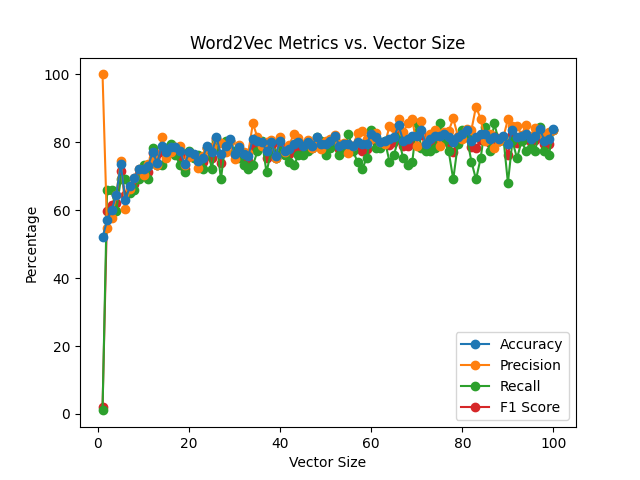
\includegraphics[width=0.4\columnwidth]{w2v_nn_vector_size_plot.png}
\end{figure}
$m_3$ has the best results in all four metrics of the three models.  The accuracy, precision, recall, and F1 score all increased with vector size - with an outlier of 100\% recall for a vector size of 1 and 100\% precision for a vector size close to 1. The size of the vector increasing means there are more dimensions to work with, and more potential relations with other word vectors to be had, allowing for more detailed predictions.\\

\item Suppose we use word2vec to train word vectors with window size as 3. Given a sentence “Very good drama”, it will be transferred to the training set with instances X and corresponding labels Y. If we choose skip-gram style, what are X and Y in the training set? If we choose CBOW style, what are X and Y in the training set?\\

The skip-gram style predicts surrounding words given a target word. In the training set, X and Y would be the following:
\begin{lstlisting}
x: ['very', 'good', 'drama']
y: [['good'], ['very', 'drama'], ['good']]
\end{lstlisting}
The CBOW style predicts a target word given surrounding words. X and Y would be the following:
\begin{lstlisting}
x: [['good', 'drama'], ['very', 'drama'], ['very', 'good']]
y: ['very', 'good', 'drama']
\end{lstlisting}

\end{enumerate}
\newpage
\section{Text Annotation}
\begin{enumerate}
\item When there is no (enough) labelled corpus to train a machine learning based NLP model, we need to create a training text dataset as golden standard through manual annotation. Choose a text annotation tool to finish the following two text annotation tasks:\\

\noindent Entity Annotation:\\ “\textit{Barack Obama was the 44th President of the United States. He was born in Hawaii and studied law at Harvard University.}”\\

Annotation Results: \\
\textit{Barack Obama} PERSON\\
\textit{44th} CARDINAL\\
\textit{the United States} GPE\\
\textit{Hawaii} GPE\\
\textit{Harvard University} ORG\\

Sentiment Annotation: “\textit{De Niro has the ability to make every role he portrays into acting gold. He gives a great performance in this film and there is a great scene where he has to take his father to a home for elderly people because he can't care for him anymore that will break your heart. I will say you won't see much bette acting anywhere.}”\\
Annotation Results: Positive\\

Report the name of the tool you chose. When you are annotating, make a couple of screenshots and put them into the report. After annotation, you should obtain a file with annotation information from the tool: the annotated data file. Submit the annotated data files for the above two tasks.
\begin{multicols}{2}
The tool used for entity annotaion is \url{termitexpert.in/annotation_spacy_ner}
\begin{center}
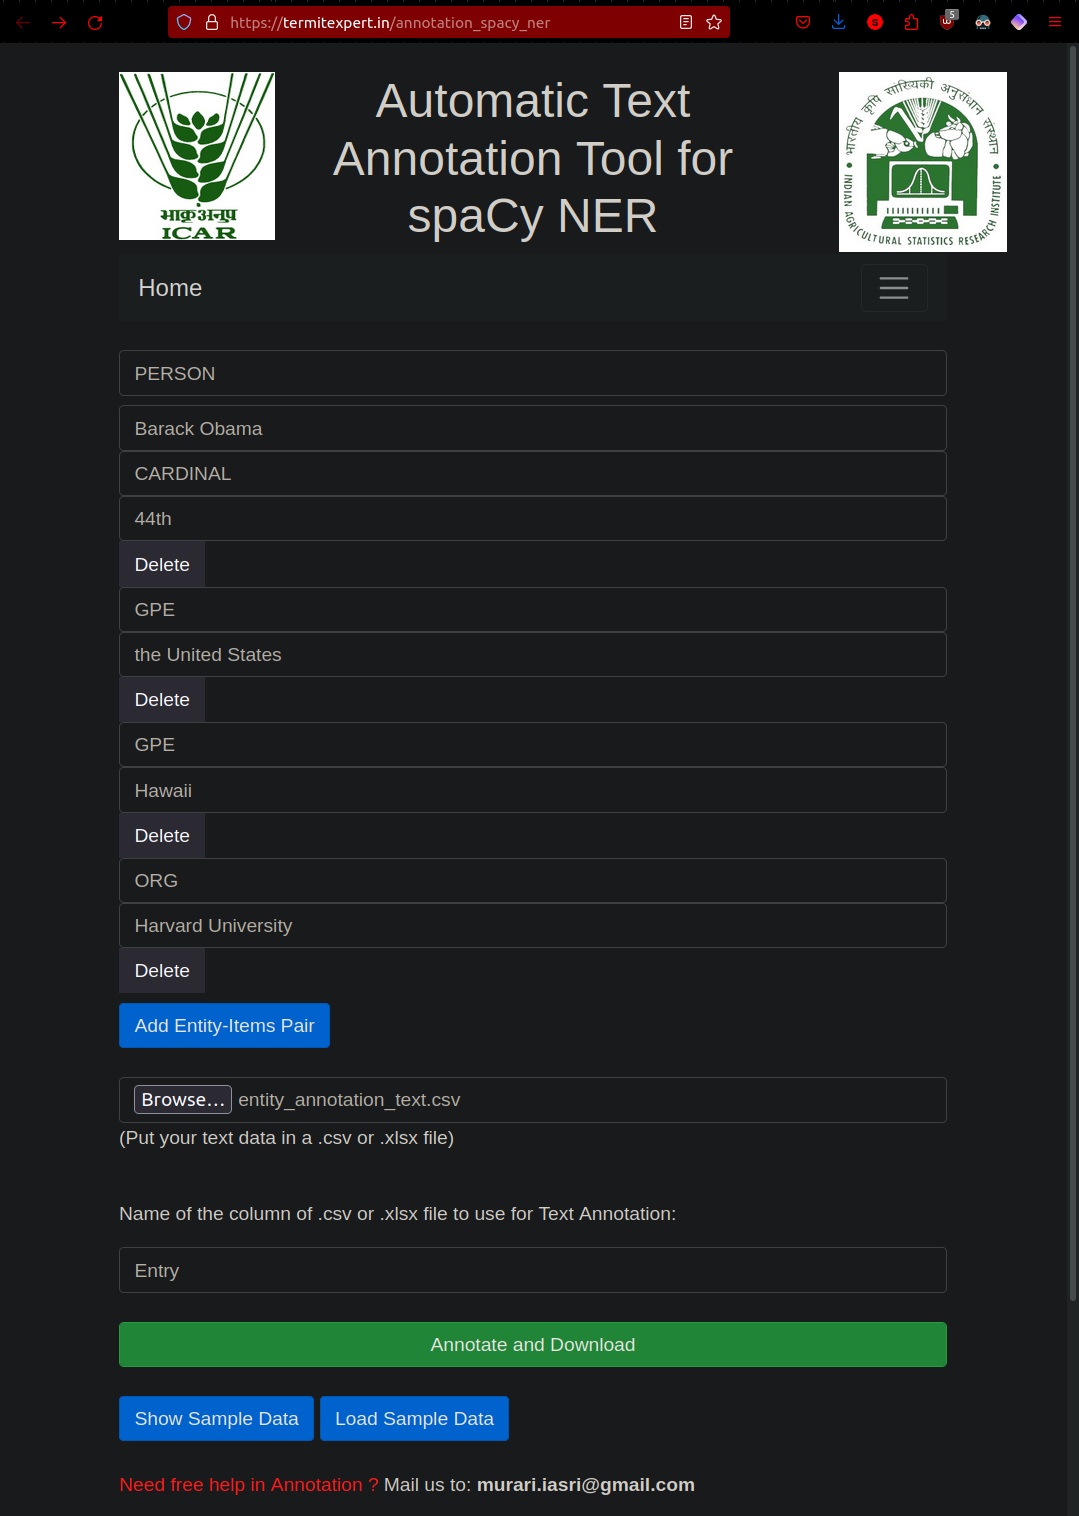
\includegraphics[scale=0.2]{entity_annotation_screenshot.png}
\end{center}
It produces a text file with the following contents:\\
\begin{lstlisting}
[('Barack Obama was the 44th President of the United States. He was born in Hawaii and studied law at Harvard University. ', {'entities': [(0, 12, 'PERSON'), (21, 25, 'CARDINAL'), (73, 79, 'GPE'), (99, 117, 'ORG')]})]
\end{lstlisting}
\end{multicols}

\newpage

The tool used for sentiment annotation is \url{https://monkeylearn.com/sentiment-analysis-online/}. I could not find any tool that gave a file as an output, but it rated the text as positive with 97.6\% confidence.
\begin{center}
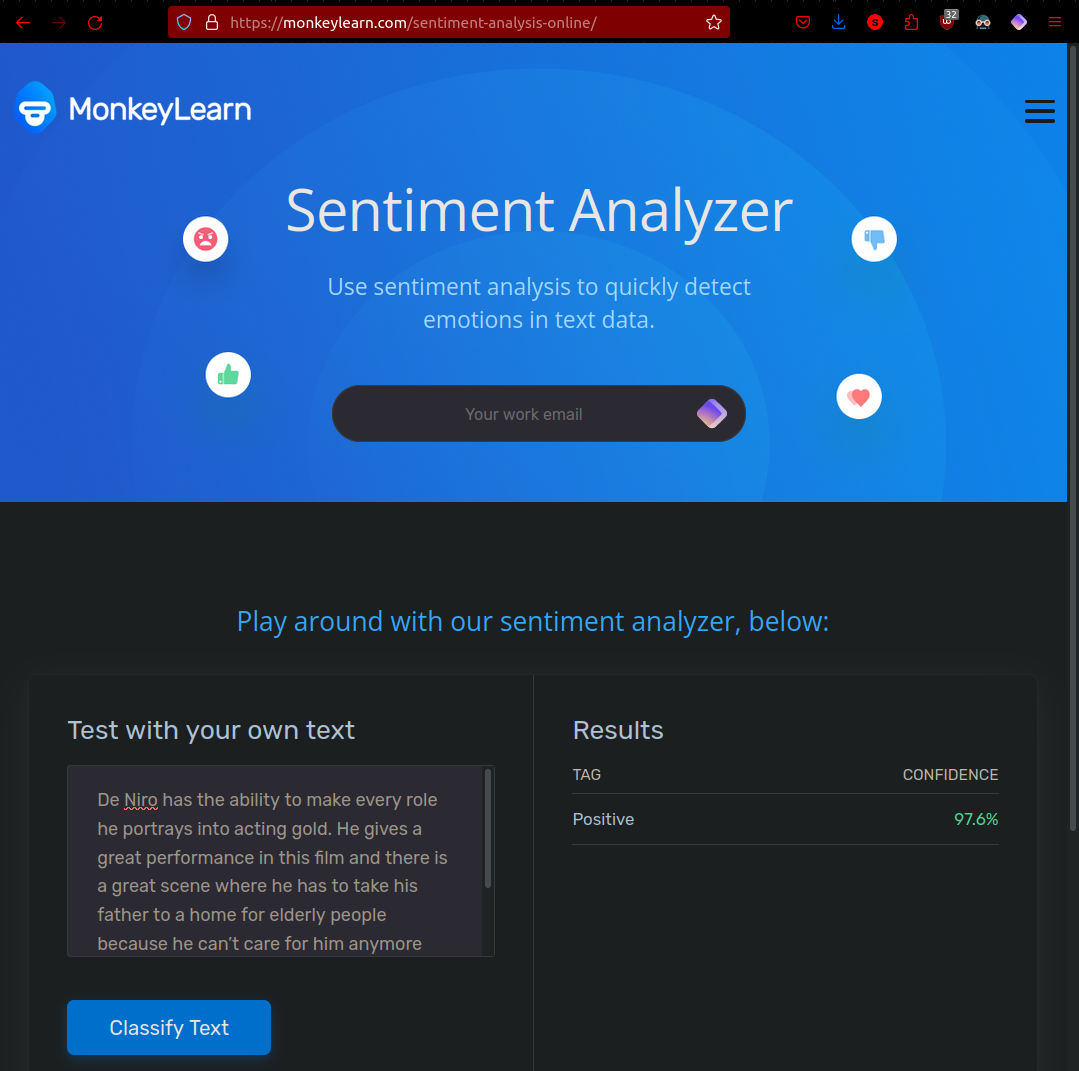
\includegraphics[scale=0.4]{sentiment_annotation_screenshot.png}
\end{center}

\newpage
\item Active learning is a method to improve annotation efficiency. The following code imitates an active learning process.
\begin{center}
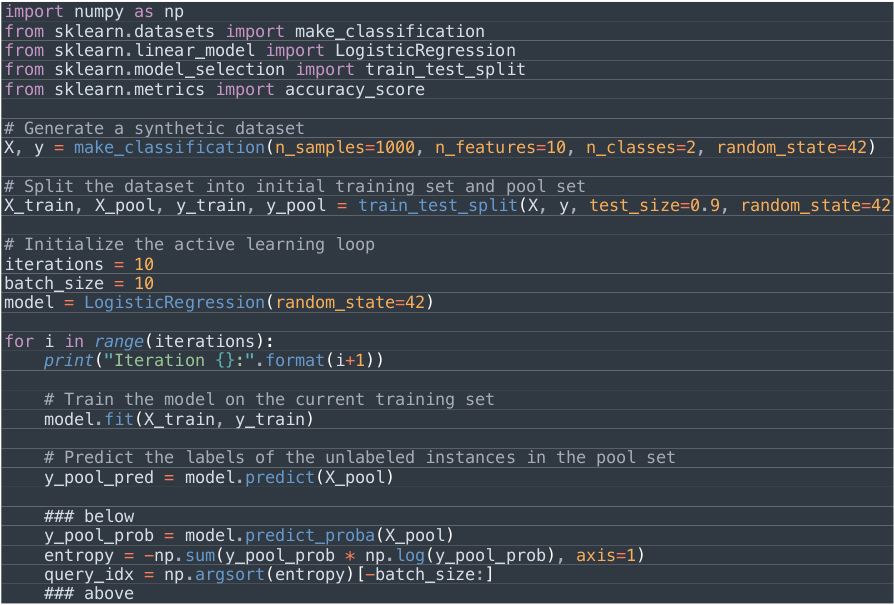
\includegraphics[scale=0.25]{HW 02 code (1).png}
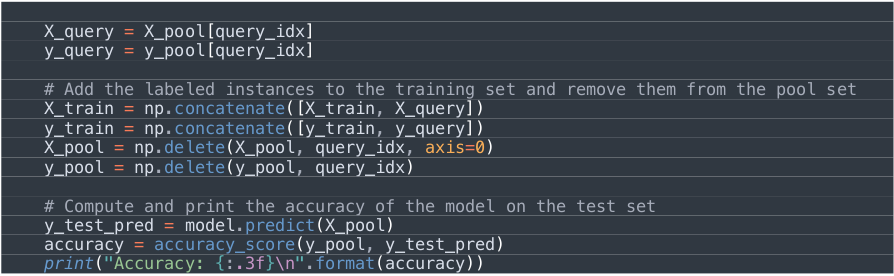
\includegraphics[scale=0.25]{HW 02 code (2).png}
\end{center}
\begin{enumerate}
\item What is the purpose of the code between “\verb"### below"” and “\verb"### above"”? Replace these code and other necessary code (as few as possible) to implement the active learning method in another strategy. Compare these two strategies, which one is better in this example?\\

The purpose of the three lines of code is to prepare to remove the values in \verb"x_pool" and \verb"y_pool" with the largest probability entropies, where entropy is a measure of randomness of the probabilities.
\begin{itemize}
\item \verb"y_pool_prob = model.predict_proba(x_pool)"\\
This line uses a logistic regression model to predict the probabilites of \verb"x_pool" and stores them in \verb"y_pool_prob".

\item \verb"entropy = -np.sum(y_pool_prob * np.log(y_pool_prob), axis=1)"\\
This line calculates the entropy of each value in the \verb"y_pool_prob".

\item \verb"query_idx = np.argsort(entropy)[-batch_size:]"\\
\verb"np.argsort" sorts the entropy list numerically and returns the original indices of the sorted values. \verb"[-batch_size]" takes the last $n$ elements, where $n=$ \verb"batch_size", of the array of indices produced by \verb"np.argsort" and stores those last indices in \verb"query_idx" to be used for selecting elements based on their indices in the next two lines.\\
\end{itemize}

replacing the last two lines of code between \verb"### below" and \verb"### above" with:
\begin{lstlisting}
least_confidence = [np.max(y_pool_prob) - np.average(prob_val) for prob_val in y_pool_prob]
query_idx = np.argsort(least_confidence)[-batch_size:]
\end{lstlisting}
calculates the least confidence, or the difference of $x$ probability in the list from the maximum probability, and takes the lowest $n$ (batch size) items in the list to be removed after being set equal to \verb"query_idx". Surprisingly, the accuracy values produced by each iteration are exactly the same as before the change. Altering the batch size by increasing it has more effect, although an increased batch size with either removal method still produced the exact same accuracies for both methods.\\


\item If the code is used for movie review annotation, how many reviews need to be labelled by the annotator every time? Discuss the possible pros and cons by increasing and decreasing this number.\\

The current batch size is 10, so 10 movie reviews would need to be labelled by the annotator each time. This helps reduce the time spent annotating, but may lower accuracy. If the batch size is increased, more reviews will need to be labelled which is more time consuming on a large scale dataset, but the accuracy would be increase as the batch size increases.

\end{enumerate}
\end{enumerate}

\end{document}
